\documentclass{ctexart}
\usepackage{PhysicalChemistryNote}

\begin{document}\pagestyle{plain}
\noindent\tbf{\LARGE 4D 多组分系统的相变与相图}\vspace{15pt}\\
\indent 在经历了漫长的对溶液的讨论后,我们终于来到了多组分系统与相图这一节.%
尽管我们没有对多组分系统相变的规律进行总结,不过我们在\tbf{4C}已经不计其数地使用了多组分系统相平衡的条件.%
因此,本节事实上没有多少新的知识,更多的是总结与归纳,以及引入一些新的方法描述多组分系统各相的平衡情况.\vspace{12pt}\\
\Section{4D.1 多组分系统的相律}
\indent 我们已经在\tbf{4A.1.7}中不加证明地给出了单组分系统的相律.对于更一般的多组分系统,%
我们也需要给定一定数量的状态函数(例如温度$T$,压力$p$等等)来确定系统的状态.%
可以想见,需要给定的条件数应当与系统中的组分数和相数都有关系.下面我们来确定其具体关系式.
\begin{derivation}
    考虑某个平衡的系统,组分数为$S$,相数为$\varPhi$,并且假定各组分在每个相中都存在,且不发生化学反应.\\
    采取摩尔分数$x_i$表示每个相的组成.因为有$\displaystyle\sum_{i=1}^{k}x_i=1$的限制存在,%
    于是每个相都需要$S-1$个独立的变量以描述其组成.由于相数为$\varPhi$,再加上相平衡时各相的温度$T$和压力$p$,%
    就需要$\varPhi(S-1)+2$个变量描述该系统.\\
    然而,由于我们需要保证各组分在各相中的化学势$\mu$相等,于是就有
    \[\mu_{i,\alpha}=\mu_{i,\beta}=\cdots=\mu_{i,\phi}(i=1,2,\cdots,S)\]
    其中$\alpha,\beta,\cdots,\phi$为系统的所有$\varPhi$个相.\\
    由于化学势是温度$T$,压力$p$和摩尔分数$x_i$的函数,因此对于每个$i$,只需任意地确定某一相$\lambda$中的$x_{i,\lambda}$,%
    就可以通过上述等量关系求得所有相中的$x_i$.因此,对于每个组分$i$,上述等式意味着$\varPhi-1$个需要满足的等量关系,一共就有$S(\varPhi-1)$个需要满足的等量关系.\\
    每个等量关系都可以使我们描述系统的独立变量减少$1$个.根据自由度的定义,就有
    \[f=\left(\varPhi(S-1)+2\right)-\left(S(\varPhi-1)\right)=S-\varPhi+2\]
    稍作整理,就可得
    \[\varPhi+f=S+2\]
    推广而言,如果某一组分$i$在某一相$\lambda$中不存在,那么$x_{i,\lambda}$就不需要被描述,保证化学势相等的等量关系也减少一个.%
    这样,变量数和等量关系同步减少,对我们的结论没有影响.
\end{derivation}
\begin{theorem}[4D.1.1 简单多组分系统的相律]
    对于一个不发生化学反应的系统,其自由度$f$满足
    \[\varPhi+f=S+2\]
    其中$S$为系统的组分数,$\varPhi$为系统的相数.
\end{theorem}
对于可能发生化学反应的系统,根据我们在普通化学中学过的知识可知一个平衡相当于一个等量关系,%
相当于这些组分之间并不独立.为此,我们需要把组分数$S$改写成独立组分数$C$,即总的组分数减去需要满足的平衡关系数.\\
\indent 对于凝聚态系统(例如具有很低的蒸气压的液体和固体),压力对系统的改变可以忽略,此时等式右边的$2$也可以改写为$1$.\\
\indent 总结上述讨论,我们可以得出相律的更一般的形式,它由Gibbs在1877年首次提出.
\begin{theorem}[4D.1.2 Gibbs相律]
    多组分系统的自由度$f$满足
    \[\varPhi+f=C+n\]
    其中$C$为系统的\tbf{独立组分数},$\varPhi$为系统的相数,$n$为外界因素的数目(多数时候取$2$,代表温度$T$和压力$p$;%
    如果压力对系统影响可忽略不计,那么也可以取$n=1$).
\end{theorem}
Gibbs相律是我们描述多组分系统的相图时所应当遵守的基本规律.\\
\indent 对于双组分系统,$S=2$,就有$f=4-\varPhi$.由于我们讨论的系统至少有一个相,%
因此,系统的状态可以用至多三个变量来确定.我们一般采取温度$T$,压力$p$和组成$x$描述其状态,%
这样系统的相图就是一个具有三个坐标轴的立体图.\\
\indent 实际情况中,我们常常采取固定某一变量的方法描述双组分系统的相图(即上述立体图的截面).%
通常来说,我们会使用$p-x$图和$T-x$图描述系统的状态.我们将在接下来的几节中介绍各种双组分系统的相图.\vspace{12pt}\\
\Section{4D.2 双组分溶液的相图}
\Part{双组分理想溶液的相图}
\indent 我们先讨论$p-x$图.
\begin{derivation}
    根据Raoult定律,组分$A$和组分$B$形成的理想溶液满足
    \[\left\{\begin{array}{l}
        p_A=p_A^\ast x_{A,\l}\\
        p_B=p_B^\ast\left(1-x_{A,\l}\right)
    \end{array}\right.\]
    于是总蒸气压
    \[p=p_A+p_B=p_B^\ast+\left(p_A^\ast-p_B^\ast\right)x_{A,\l}\]
    如果我们以$x_{A,\l}$为横轴,$p$为纵轴,就可以得到如下的相图.
    \begin{center}
        \documentclass{standalone}
\usepackage{PhysicalChemistryNote}
\begin{document}
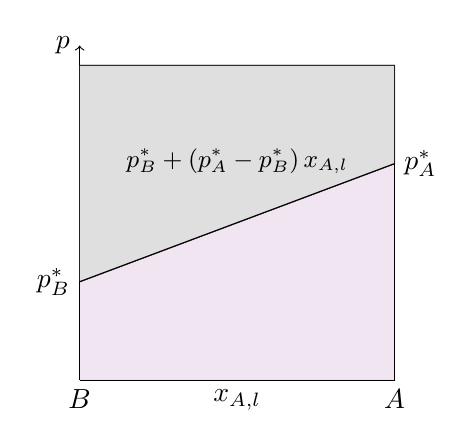
\begin{tikzpicture}
    \draw[-] (0,0) -- (4,0);
    \draw[->] (0,0) -- (0,4.25) node[left]{$p$};
    \draw[-] (4,0) -- (4,4);
    \draw[-] (0,4) -- (4,4);
    \node[below] at (0,0) {$B$};
    \node[below] at (4,0) {$A$};
    \node[below] at (2,0) {$x_{A,\l}$};
    \filldraw[fill=lightgray,opacity=0.5] (0,1.25) -- (4,2.75) -- (4,4) -- (0,4);
    \filldraw[fill=violet,opacity=0.1] (0,1.25) -- (4,2.75) -- (4,0) -- (0,0);
    \node[left] at (0,1.25) {$p_B^\ast$};
    \node[right] at (4,2.75) {$p_A^\ast$};
    \node[above] at (2,2.5) {\small{$p_B^\ast+\left(p_A^\ast-p_B^\ast\right)x_{A,\l}$}};
    \draw[-] (0,1.25) -- (4,2.75);
    
\end{tikzpicture}
\end{document}
    \end{center}
    可以看到,选取某组分在液相中的摩尔分数$x_\l$和压力$p$,%
    作出的理想溶液相图中两相的分界线为直线.%
    其中上面灰色的部分为液相,下面紫色的部分却是意义尚且不明的.事实上,紫色的部分中有一块区域是气-液共存相,而另一部分则为气相(在只有气相时$x_{A,\l}$也就失去意义).%
    我们将在介绍$T-x_{A,\g}$图后详细阐明这一点.\\
    显而易见的,两种组分在气相中的含量与它们在液相中的含量并不相同.我们有
    \[x_{A,\g}=\dfrac{p_A}{p}=\dfrac{p_A^\ast x_{A,\l}}{p_B^\ast+\left(p_A^\ast-p_B^\ast\right)x_{A,\l}}\]
    于是
    \[x_{A,\l}=\dfrac{p_B^\ast x_{A,\g}}{p_A^\ast+\left(p_B^\ast-p_A^\ast\right)x_{A,\g}}\]
    从而
    \[p=p_B^\ast+\dfrac{p_B^\ast x_{A,\g}\left(p_A^\ast-p_B^\ast\right)}{p_A^\ast+\left(p_B^\ast-p_A^\ast\right)x_{A,\g}}
    =\dfrac{p_A^\ast p_B^\ast}{p_A^\ast+\left(p_B^\ast-p_A^\ast\right)x_{A,\g}}\]
    我们以$x_{A,\g}$为横轴,$p$为纵轴,可以得到如下的相图.
    \begin{center}
        \documentclass{standalone}
\usepackage{PhysicalChemistryNote}
\begin{document}
\begin{tikzpicture}
    \draw[-] (0,0) -- (4,0);
    \draw[->] (0,0) -- (0,4.25) node[left]{$p$};
    \draw[-] (4,0) -- (4,4);
    \draw[-] (0,4) -- (4,4);
    \node[below] at (0,0) {$B$};
    \node[below] at (4,0) {$A$};
    \node[below] at (2,0) {$x_{A,\g}$};
    \draw[domain=0:4] plot[smooth](\x,{4*1.25*2.75/(11-1.5*\x)});
    \filldraw[fill=lightgray,opacity=0.5,domain=0:4] plot[smooth](\x,{4*1.25*2.75/(11-1.5*\x)}) -- (4,4) -- (0,4);
    \filldraw[fill=violet,opacity=0.1,domain=0:4] plot[smooth](\x,{4*1.25*2.75/(11-1.5*\x)}) -- (4,0) -- (0,0);
    \node[left] at (0,1.25) {$p_B^\ast$};
    \node[right] at (4,2.75) {$p_A^\ast$};
    \node[below] at (2,1.5) {\small{$\dfrac{p_A^\ast p_B^\ast}{p_A^\ast+\left(p_B^\ast-p_A^\ast\right)x_{A,\g}}$}};
    
    
\end{tikzpicture}
\end{document}
    \end{center}
    可以看到,以气相中$A$的摩尔分数作出的相图的分界线是一条下凹的曲线,总是处于液相线之下.如果我们把两条线画在同一张图中,就有
    \begin{center}
        \documentclass{standalone}
\usepackage{PhysicalChemistryNote}
\begin{document}
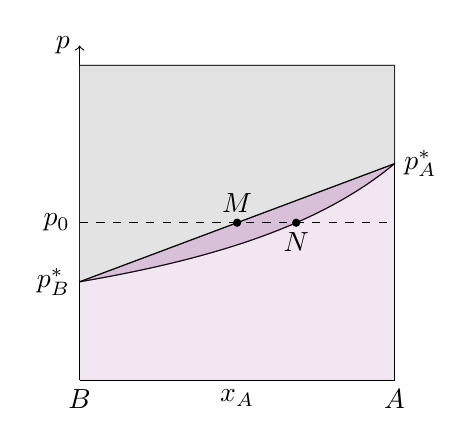
\begin{tikzpicture}
    \draw[-] (0,0) -- (4,0);
    \draw[->] (0,0) -- (0,4.25) node[left]{$p$};
    \draw[-] (4,0) -- (4,4);
    \draw[-] (0,4) -- (4,4);
    \node[below] at (0,0) {$B$};
    \node[below] at (4,0) {$A$};
    \node[below] at (2,0) {$x_{A}$};
    \draw[domain=0:4] plot[smooth](\x,{4*1.25*2.75/(11-1.5*\x)});
    \filldraw[fill=lightgray,opacity=0.25,domain=0:4] plot[smooth](\x,{4*1.25*2.75/(11-1.5*\x)}) -- (4,4) -- (0,4);
    \filldraw[fill=violet,opacity=0.05,domain=0:4] plot[smooth](\x,{4*1.25*2.75/(11-1.5*\x)}) -- (4,0) -- (0,0);
    \filldraw[fill=lightgray,opacity=0.25] (0,1.25) -- (4,2.75) -- (4,4) -- (0,4);
    \filldraw[fill=violet,opacity=0.05] (0,1.25) -- (4,2.75) -- (4,0) -- (0,0);
    \filldraw[fill=violet,opacity=0.15,domain=0:4] plot[smooth](\x,{4*1.25*2.75/(11-1.5*\x)})--(0,1.25);
    \node[left] at (0,1.25) {$p_B^\ast$};
    \node[left] at (0,2) {$p_0$};
    \node[right] at (4,2.75) {$p_A^\ast$};
    \draw[-] (0,1.25) -- (4,2.75);
    \draw[dashed] (0,2) -- (4,2);
    \fill (2,2) circle (1.5pt) node[above]{$M$};
    \fill (2.75,2) circle (1.5pt) node[below]{$N$};
    
\end{tikzpicture}
\end{document}
    \end{center}
    在此我们有必要解释梭形区域(即图中颜色加深的部分)的物理意义.前面已经说到在$p-x_{A,\l}$线(也称为液相线)之上的区域一定是纯液相,%
    同样地也可以知道在$p-x_{A,\g}$线(也称为气相线)之下的区域一定是纯气相,而中间的梭形区域就是液相和气相共存的区域.\\
    根据相律,在梭形区域两相平衡,系统的自由度为$f=C+n-\varPhi=2+2-0$,只要给定压强$p_0$和温度$T$就可以确定其组成和状态.%
    因此,如果给定系统中$A$的总含量$x_{A}$和压力$p_0$,如果作一条直线$p=p_0$分别交两条分界线于$M,N$两点,%
    满足$x_M<x_A<x_N$,那么此时系统就存在气液两相,液相的成分就是$M$点,而气相的成分就是$N$点.当$x_A$在上述范围内变动时,液相和气相的组成都不变,但是物质的量之比会发生变化.\\
    从上面的图中也容易看出在平衡时,蒸气压大的组分在气相中的摩尔分数总是比在液相中的摩尔分数高.
\end{derivation}
通常来说,我们更常在恒定压力下对系统进行改变,例如蒸馏和精馏等操作.%
因此,$T-x$图更为常用.
\begin{derivation}\setcounter{equation}{0}
    我们仍然讨论由组分$A$和组分$B$组成的理想溶液,并保持总压力为$p$不变.\\
    根据Clausius-Clapeyron方程有
    \begin{equation}
        \dfrac{\di\ln p_{i}^\ast}{\di T}=\dfrac{\Delta_\vap H_{\m,i}}{RT^2}
    \end{equation}
    其中$i=A,B$.我们再假定摩尔蒸发焓随温度变化很小,设纯的$i$在$p$下的沸点为$T_i^\ast$,对(1)定积分有
    \begin{equation}
        \ln\dfrac{p_i^\ast}{p}=\dfrac{\Delta_\vap H_{\m,i}}{R}\left(\dfrac{1}{T_i^\ast}-\dfrac1T\right)
    \end{equation}
    移项并取指数就有
    \begin{equation}
        p_i^\ast=p\exp{\left[\dfrac{\Delta_\vap H_{\m,i}}{R}\left(\dfrac{1}{T_i^\ast}-\dfrac1T\right)\right]}
    \end{equation}
    根据Raoult定律有
    \begin{equation}
        p=p_{A}^\ast x_{A,\l}+p_B^\ast\left(1-x_{A,\l}\right)
    \end{equation}
    将(3)代入其中就有
    \begin{equation}
        x_{A,\l}\exp{\left[\dfrac{\Delta_\vap H_{\m,A}}{R}\left(\dfrac{1}{T_A^\ast}-\dfrac1T\right)\right]}
        +\left(1-x_{A,\l}\right)\exp{\left[\dfrac{\Delta_\vap H_{\m,B}}{R}\left(\dfrac{1}{T_B^\ast}-\dfrac1T\right)\right]}=1
    \end{equation}
    这就给出了$T$与$x_{A,\l}$的函数关系,绘制出的相图如下所示.
    \begin{center}
        \documentclass{standalone}
\usepackage{PhysicalChemistryNote}
\begin{document}
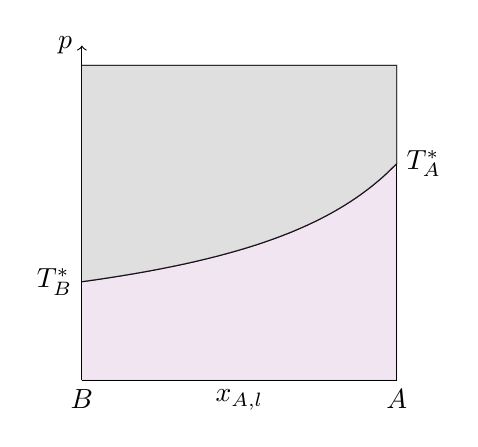
\begin{tikzpicture}
    \draw[-] (0,0) -- (4,0);
    \draw[->] (0,0) -- (0,4.25) node[left]{$p$};
    \draw[-] (4,0) -- (4,4);
    \draw[-] (0,4) -- (4,4);
    \node[below] at (0,0) {$B$};
    \node[below] at (4,0) {$A$};
    \node[below] at (2,0) {$x_{A,\l}$};
    \draw[domain=0:4] plot[smooth](\x,{1/ln(0.1967*(11.3117-\x))});
    \filldraw[fill=lightgray,opacity=0.5,domain=0:4] plot[smooth](\x,{1/ln(0.1967*(11.3117-\x))}) -- (4,4) -- (0,4);
    \filldraw[fill=violet,opacity=0.1,domain=0:4] plot[smooth](\x,{1/ln(0.1967*(11.3117-\x))}) -- (4,0) -- (0,0);
    \node[left] at (0,1.25) {$T_B^\ast$};
    \node[right] at (4,2.75) {$T_A^\ast$}; 
    
\end{tikzpicture}
\end{document}
    \end{center}
    现在我们仍尝试用$x_{A,\g}$来代替$x_{A,\l}$作出相图.在推导$p-x$图时我们已经知道
    \begin{equation}
        p=\dfrac{p_A^\ast p_B^\ast}{p_A^\ast+\left(p_B^\ast-p_A^\ast\right)x_{A,\g}}
    \end{equation}
    将(3)代入(6)就有
    \begin{equation}
        \dfrac{1-x_{A,\g}}{\exp{\left[\dfrac{\Delta_\vap H_{\m,B}}{R}\left(\dfrac{1}{T_B^\ast}-\dfrac1T\right)\right]}}+
        \dfrac{x_{A,\g}}{\exp{\left[\dfrac{\Delta_\vap H_{\m,A}}{R}\left(\dfrac{1}{T_A^\ast}-\dfrac1T\right)\right]}}=1
    \end{equation}
    这就给出了$T$与$x_{A,\g}$的函数关系,绘制出的相图如下所示.
    \begin{center}
        \documentclass{standalone}
\usepackage{PhysicalChemistryNote}
\begin{document}
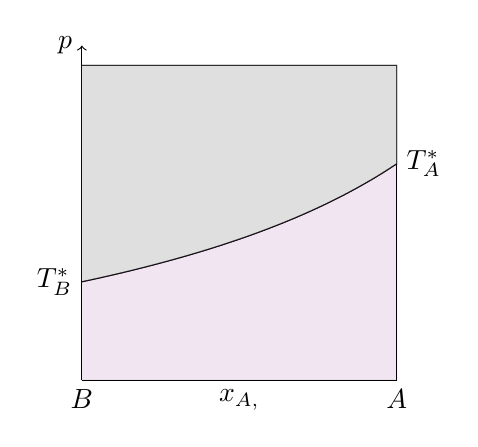
\begin{tikzpicture}
    \draw[-] (0,0) -- (4,0);
    \draw[->] (0,0) -- (0,4.25) node[left]{$p$};
    \draw[-] (4,0) -- (4,4);
    \draw[-] (0,4) -- (4,4);
    \node[below] at (0,0) {$B$};
    \node[below] at (4,0) {$A$};
    \node[below] at (2,0) {$x_{A,\g}$};
    \draw[domain=0:4] plot[smooth](\x,{-1/ln(-0.06145*(-7.3117-\x))});
    \filldraw[fill=lightgray,opacity=0.5,domain=0:4] plot[smooth](\x,{-1/ln(-0.06145*(-7.3117-\x))}) -- (4,4) -- (0,4);
    \filldraw[fill=violet,opacity=0.1,domain=0:4] plot[smooth](\x,{-1/ln(-0.06145*(-7.3117-\x))}) -- (4,0) -- (0,0);
    \node[left] at (0,1.25) {$T_B^\ast$};
    \node[right] at (4,2.75) {$T_A^\ast$}; 
    
\end{tikzpicture}
\end{document}
    \end{center}
    你可能觉得两张图看起来并没有什么区别.为了方便演示,我们将它们放在同一幅图中,即下面左边的相图.
    \begin{center}
        \documentclass{standalone}
\usepackage{PhysicalChemistryNote}
\begin{document}
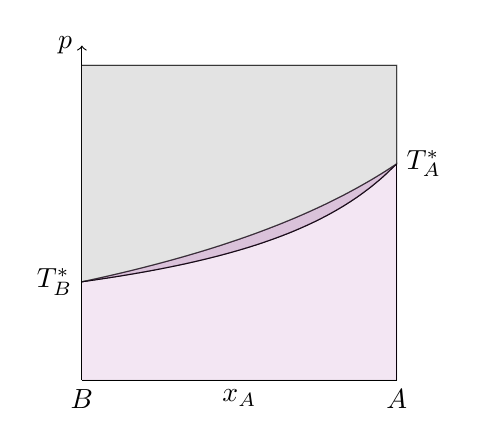
\begin{tikzpicture}
    \draw[-] (0,0) -- (4,0);
    \draw[->] (0,0) -- (0,4.25) node[left]{$p$};
    \draw[-] (4,0) -- (4,4);
    \draw[-] (0,4) -- (4,4);
    \node[below] at (0,0) {$B$};
    \node[below] at (4,0) {$A$};
    \node[below] at (2,0) {$x_{A}$};
    \draw[domain=0:4] plot[smooth](\x,{{-1/ln(-0.06145*(-7.3117-\x))}});
    \draw[domain=0:4] plot[smooth](\x,{1/ln(0.1967*(11.3117-\x))});
    \filldraw[fill=lightgray,opacity=0.25,domain=0:4] plot[smooth](\x,{-1/ln(-0.06145*(-7.3117-\x))}) -- (4,4) -- (0,4);
    \filldraw[fill=violet,opacity=0.05,domain=0:4] plot[smooth](\x,{-1/ln(-0.06145*(-7.3117-\x))}) -- (4,0) -- (0,0);
    \filldraw[fill=lightgray,opacity=0.25,domain=0:4] plot[smooth](\x,{1/ln(0.1967*(11.3117-\x))}) -- (4,4) -- (0,4);
    \filldraw[fill=violet,opacity=0.05,domain=0:4] plot[smooth](\x,{1/ln(0.1967*(11.3117-\x))}) -- (4,0) -- (0,0);
    \filldraw[fill=violet,opacity=0.15] plot[smooth,domain=0:4](\x,{{-1/ln(-0.06145*(-7.3117-\x))}})--plot[smooth,domain=4:0](\x,{1/ln(0.1967*(11.3117-\x))});
    \node[left] at (0,1.25) {$T_B^\ast$};
    \node[right] at (4,2.75) {$T_A^\ast$};
\end{tikzpicture}
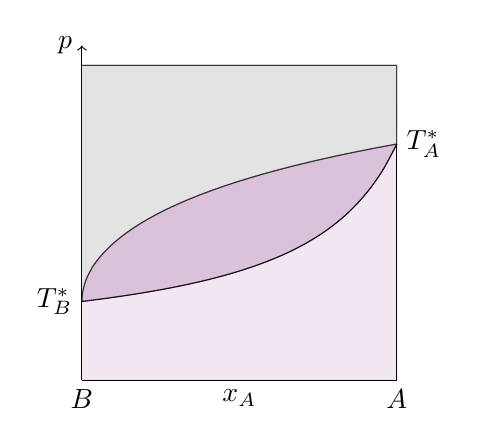
\begin{tikzpicture}
    \draw[-] (0,0) -- (4,0);
    \draw[->] (0,0) -- (0,4.25) node[left]{$p$};
    \draw[-] (4,0) -- (4,4);
    \draw[-] (0,4) -- (4,4);
    \node[below] at (0,0) {$B$};
    \node[below] at (4,0) {$A$};
    \node[below] at (2,0) {$x_{A}$};
    \draw[domain=0:4,samples=500] plot[smooth](\x,{(\x^0.5*(e^(-\x/6)/2+1))/1.2567+1});
    \draw[domain=0:4] plot[smooth](\x,{1/ln(0.25*(4*e+e^(1/3)*\x-e*\x))});
    \filldraw[fill=lightgray,opacity=0.25,domain=0:4,samples=500] plot[smooth](\x,{(\x^0.5*(e^(-\x/6)/2+1))/1.2567+1}) -- (4,4) -- (0,4);
    \filldraw[fill=violet,opacity=0.05,domain=0:4,samples=500] plot[smooth](\x,{(\x^0.5*(e^(-\x/6)/2+1))/1.2567+1}) -- (4,0) -- (0,0);
    \filldraw[fill=lightgray,opacity=0.25,domain=0:4] plot[smooth](\x,{1/ln(0.25*(4*e+e^(1/3)*\x-e*\x))}) -- (4,4) -- (0,4);
    \filldraw[fill=violet,opacity=0.05,domain=0:4] plot[smooth](\x,{1/ln(0.25*(4*e+e^(1/3)*\x-e*\x))}) -- (4,0) -- (0,0);
    \filldraw[fill=violet,opacity=0.15] plot[smooth,domain=0:4](\x,{1/ln(0.25*(4*e+e^(1/3)*\x-e*\x))}) -- plot[smooth,domain=4:0,samples=500](\x,{(\x^0.5*(e^(-\x/6)/2+1))/1.2567+1});
    \node[left] at (0,1) {$T_B^\ast$};
    \node[right] at (4,3) {$T_A^\ast$};
\end{tikzpicture}
\end{document}
    \end{center}
    这和你以往见到的$T-x$图似乎有所不同,因为两条线都是下凸的.不要着急,我们再稍稍调整一下$A$与$B$的蒸发焓之比,就可以得到上面右边的相图.%
    这就与我们常常见到的$T-x$图相一致了\footnotemark.%
    我们不难发现,这里的液相线总是在气相线的下方,这与$p-x$图恰好相反.\\
    我们将用此图来解释很多重要操作的原理.
\end{derivation}\footnotetext{其实右图并不是精确绘制的,因为表达式太过冗长,于是笔者采取了一些小小的简化,至少形状看着像就行.}
\Part{蒸馏和分馏的基本原理}
\indent 在有机化学实验中常常使用蒸馏和分馏方法分离沸点不同的物质.我们从$T-x$图入手对这两种体系进行简单的解释.
\begin{proof}
    我们假定待分离的混合物是由$A$和$B$组成的理想溶液.最初,溶液成分为$x_1$.%
    将其加热到温度为$T$时,溶液就应当沸腾,对应的气相中$A$的含量为$x_2$.
    \begin{center}
        \documentclass{standalone}
\usepackage{PhysicalChemistryNote}
\begin{document}
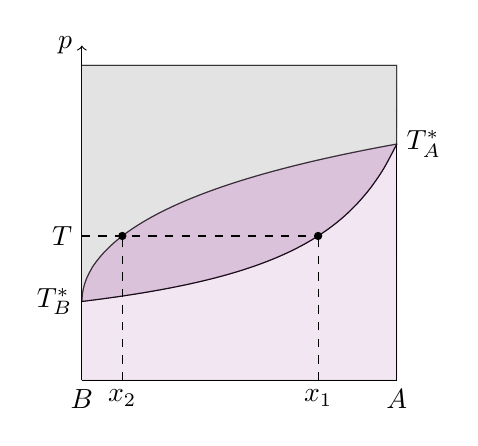
\begin{tikzpicture}
    \draw[-] (0,0) -- (4,0);
    \draw[->] (0,0) -- (0,4.25) node[left]{$p$};
    \draw[-] (4,0) -- (4,4);
    \draw[-] (0,4) -- (4,4);
    \node[below] at (0,0) {$B$};
    \node[below] at (4,0) {$A$};
    \draw[domain=0:4,samples=500] plot[smooth](\x,{(\x^0.5*(e^(-\x/6)/2+1))/1.2567+1});
    \draw[domain=0:4] plot[smooth](\x,{1/ln(0.25*(4*e+e^(1/3)*\x-e*\x))});
    \filldraw[fill=lightgray,opacity=0.25,domain=0:4,samples=500] plot[smooth](\x,{(\x^0.5*(e^(-\x/6)/2+1))/1.2567+1}) -- (4,4) -- (0,4);
    \filldraw[fill=violet,opacity=0.05,domain=0:4,samples=500] plot[smooth](\x,{(\x^0.5*(e^(-\x/6)/2+1))/1.2567+1}) -- (4,0) -- (0,0);
    \filldraw[fill=lightgray,opacity=0.25,domain=0:4] plot[smooth](\x,{1/ln(0.25*(4*e+e^(1/3)*\x-e*\x))}) -- (4,4) -- (0,4);
    \filldraw[fill=violet,opacity=0.05,domain=0:4] plot[smooth](\x,{1/ln(0.25*(4*e+e^(1/3)*\x-e*\x))}) -- (4,0) -- (0,0);
    \filldraw[fill=violet,opacity=0.15] plot[smooth,domain=0:4](\x,{1/ln(0.25*(4*e+e^(1/3)*\x-e*\x))}) -- plot[smooth,domain=4:0,samples=500](\x,{(\x^0.5*(e^(-\x/6)/2+1))/1.2567+1});
    \node[left] at (0,1) {$T_B^\ast$};
    \node[right] at (4,3) {$T_A^\ast$};
    \draw[dashed] (3,0)--(3,1.8316);
    \draw[dashed] (0,1.8316)--(3,1.8316);
    \draw[dashed] (0.5131,0)--(0.5131,1.8316);
    \node[below] at (3,0) {$x_1$};
    \node[below] at (0.5131,0) {$x_2$};
    \node[left] at (0,1.8316) {$T$};
    \fill (3,1.8316) circle (1.5pt);
    \fill (0.5131,1.8316) circle (1.5pt);
\end{tikzpicture}
\end{document}
    \end{center}
    再将气相导出体系后冷凝,就可以得到低沸点组分$B$含量大大提高的馏分,从而实现收集(或除去)低沸点组分的操作.\\
    从上面的图中也可以看出,有时蒸馏的效果也并不好(我们只将$B$的含量从$1-x_1$提高到了$1-x_2$).这时,可以采用分馏的方法.%
    分馏的本质就是进行多次蒸馏,就像下面这样.
    \begin{center}
        \documentclass{standalone}
\usepackage{PhysicalChemistryNote}
\begin{document}
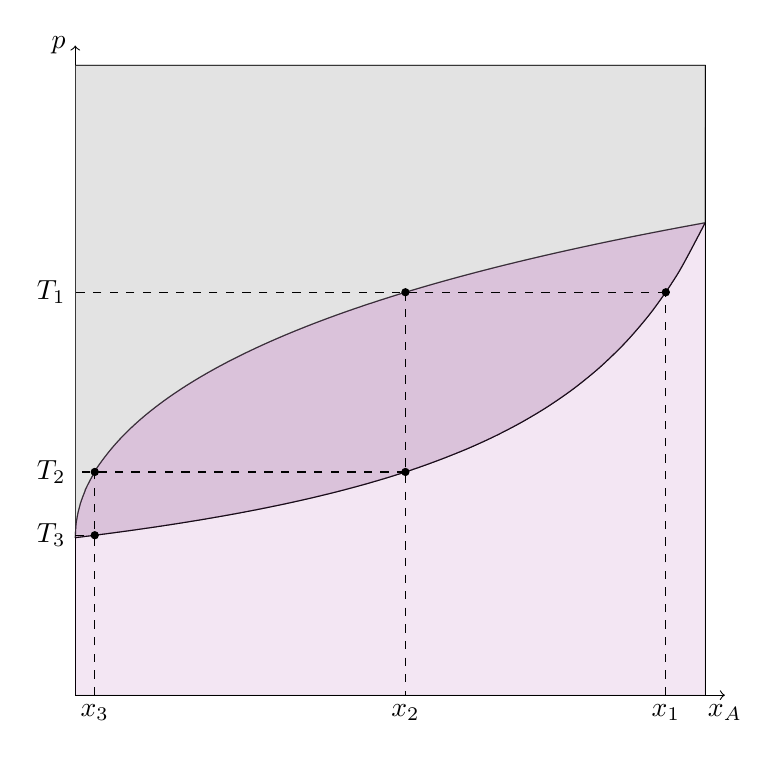
\begin{tikzpicture}
    \draw[->] (0,0) -- (8.25,0) node[below] {$x_A$};
    \draw[->] (0,0) -- (0,8.25) node[left]{$p$};
    \draw[-] (8,0) -- (8,8);
    \draw[-] (0,8) -- (8,8);
    \draw[domain=0:8,samples=1000] plot[smooth](\x,{2*((\x/2)^0.5*(e^(-\x/12)/2+1))/1.2567+2});
    \draw[domain=0:8] plot[smooth](\x,{2/ln(0.25*(4*e+e^(1/3)*(\x/2)-e*(\x/2)))});
    \filldraw[fill=lightgray,opacity=0.25,domain=0:8,samples=1000] plot[smooth](\x,{2*((\x/2)^0.5*(e^(-\x/12)/2+1))/1.2567+2}) -- (8,8) -- (0,8);
    \filldraw[fill=violet,opacity=0.05,domain=0:8,samples=1000] plot[smooth](\x,{2*((\x/2)^0.5*(e^(-\x/12)/2+1))/1.2567+2}) -- (8,0) -- (0,0);
    \filldraw[fill=lightgray,opacity=0.25,domain=0:8] plot[smooth](\x,{2/ln(0.25*(4*e+e^(1/3)*(\x/2)-e*(\x/2)))}) -- (8,8) -- (0,8);
    \filldraw[fill=violet,opacity=0.05,domain=0:8] plot[smooth](\x,{2/ln(0.25*(4*e+e^(1/3)*(\x/2)-e*(\x/2)))}) -- (8,0) -- (0,0);
    \filldraw[fill=violet,opacity=0.15] plot[smooth,domain=0:8](\x,{2/ln(0.25*(4*e+e^(1/3)*(\x/2)-e*(\x/2)))}) -- plot[smooth,domain=8:0,samples=500](\x,{2*((\x/2)^0.5*(e^(-\x/12)/2+1))/1.2567+2});
    \draw[dashed] (7.5,0)--(7.5,5.1167);
    \draw[dashed] (7.5,5.1167)--(0,5.1167);
    \draw[dashed] (4.1928,5.1167)--(4.1928,0);
    \draw[dashed] (4.1928,2.8344)--(0,2.8344);
    \draw[dashed] (0.2477,0)--(0.2477,2.8344);
    \draw[dashed] (0,2.0308)--(0.2477,2.0308);
    \node[below] at (7.5,0) {$x_1$};
    \node[below] at (4.1928,0) {$x_2$};
    \node[below] at (0.2477,0) {$x_3$};
    \node[left] at (0,5.1167) {$T_1$};
    \node[left] at (0,2.8344) {$T_2$};
    \node[left] at (0,2.0308) {$T_3$};
    \fill (7.5,5.1167) circle (1.5pt);
    \fill (4.1928,5.1167) circle (1.5pt);
    \fill (4.1928,2.8344) circle (1.5pt);
    \fill (0.2477,2.8344) circle (1.5pt);
    \fill (0.2477,2.0308) circle (1.5pt);
\end{tikzpicture}
\end{document}
    \end{center}
    我们将一步蒸馏得到的液体继续进行蒸馏操作,就可以使得到的液体中$B$的含量进一步提高.%
    在实验中,这样的操作可以通过韦氏分馏柱达成,每一步蒸馏得到的气相都将在分馏柱的更上端(温度更低处)发生冷凝,%
    此时气相中$B$的含量继续增大,向上移动,而液相中$A$的含量增大,向下流动回到反应体系中.反复这样的过程,我们就能在分馏柱的顶端得到几乎纯的$B$,%
    而最终下端的容器中得到几乎纯的$A$,从而实现对两种物质的良好的分离.
\end{proof}
\Part{双组分非理想溶液的相图与共沸混合物}
\indent 我们已经讨论了理想溶液的情况,而实际情况有时会比较复杂.%
在本节,我们主要把目光放在可以任意互溶的两种液体组成的非理想溶液上.\\
\indent 非理想溶液对理想情况的偏离与两种组分的分子间作用力是密切相关的.%
假设这两种组分为\ce{A}和\ce{B}.如果\ce{A-B}间作用力小于\ce{A-A}或\ce{B-B}间作用力,%
那么混合后分子受到的作用力减小,其蒸气压相对理想值就会偏高,沸点也相应地会降低.%
\ce{H2O}和\ce{CH3CH2OH}组成的非理想溶液就属于这一种情形.这一系统在常压下的$T-x$图如下.
\begin{figure}[H]
    \centering\documentclass{standalone}
\usepackage{PhysicalChemistryNote}
\begin{document}
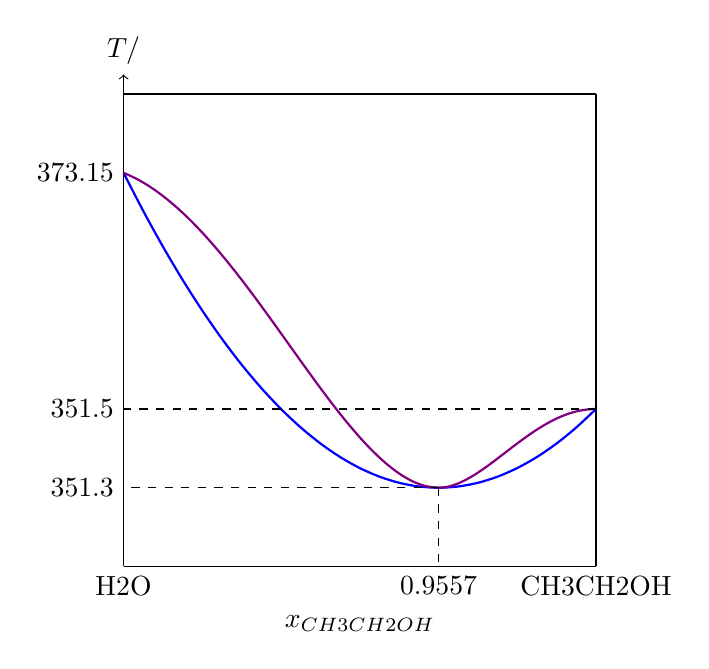
\begin{tikzpicture}
    \draw[-] (0,0) -- (6,0);
    \draw[->] (0,0) -- (0,6.25) node[above]{$T/\K$};
    \draw[-] (6,0) -- (6,6);
    \draw[-] (0,6) -- (6,6);
    \node[below] at (0,0) {{\ce{H2O}}};
    \node[below] at (6,0) {{\ce{CH3CH2OH}}};
    \node[below] at (3,-0.5) {$x_{\ce{CH3CH2OH}}$};
    \draw[domain=0:6,thick,blue] plot[smooth](\x,{(\x-4)^2/4+1});
    \draw[domain=0:4,thick,violet] plot[smooth](\x,{(\x+5)^2*(\x-4)^2/100+1});
    \draw[domain=4:6,thick,violet] plot[smooth](\x,{(\x-4)^2*(\x-8)^2/16+1});
    \draw[dashed] (4,1)--(4,0) node[below]{$0.9557$};
    \draw[dashed] (4,1)--(0,1) node[left]{$351.3\K$};
    \draw[dashed] (6,2)--(0,2) node[left]{$351.5\K$};
    \node[left] at (0,5) {$373.15\K$};
\end{tikzpicture}
\end{document}
\end{figure}
与理想溶液不同,这张$T-x$图上出现了最低点,我们称之为\tbf{最低共沸点}.在此处,气相线和液相线重合,即两相具有相同的组成.
\begin{definition}[4D.2.1 共沸]
    \tbf{共沸}(或称\tbf{恒沸})是指非理想液体混合物以特定比例组成时,%
    在一定压力下沸腾,其蒸气组成比例与溶液相同的现象.%
    共沸时,沸腾产生的蒸气与液体本身有着完全相同的组成.
\end{definition}
\begin{definition}[4D.2.2 最低共沸点]
    如果溶液达到共沸的温度低于其所有组成成分的沸点,则称该共沸温度为\tbf{最低共沸点},此时的溶液称为\tbf{最低共沸混合物}.
\end{definition}
对于上述混合物而言,达到共沸时\ce{H2O}和\ce{CH3CH2OH}的摩尔分数分别为$4.43\%$和$95.57\%$.%
参考蒸馏的原理,对组成为$0<x_{\ce{CH3CH2OH}}<0.9557$的溶液,蒸馏只能得到纯\ce{H2O}蒸汽和上述组成的共沸混合物.%
因此,如果起始时乙醇浓度不太高,我们无论如何都无法通过蒸馏得到纯的乙醇,%
只能采取别的手段(例如加入活泼金属后回流除水)来得到无水乙醇.\\
\indent 类似地,我们前面说的组分\ce{A}和\ce{B}间的作用力也可能比各自之间作用力都要大,%
那么混合后分子受到的作用力增大,其蒸气压相对理想值就会偏低,沸点也会相应升高.%
\ce{H2O}和\ce{HCl}组成的非理想溶液就属于这一种情形.这一系统在常压下的$T-x$图如下.
\begin{center}
    \documentclass{standalone}
\usepackage{PhysicalChemistryNote}
\begin{document}
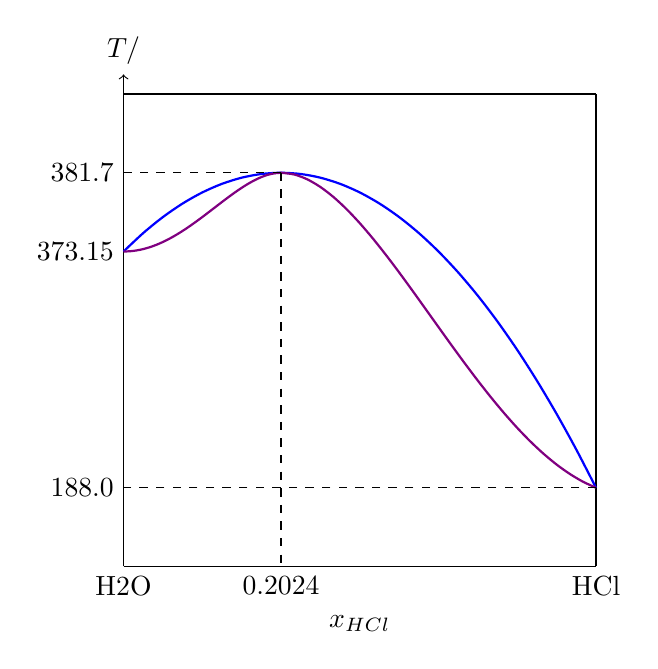
\begin{tikzpicture}
    \draw[-] (0,0) -- (6,0);
    \draw[->] (0,0) -- (0,6.25) node[above]{$T/\K$};
    \draw[-] (6,0) -- (6,6);
    \draw[-] (0,6) -- (6,6);
    \node[below] at (0,0) {{\ce{H2O}}};
    \node[below] at (6,0) {{\ce{HCl}}};
    \node[below] at (3,-0.5) {$x_{\ce{HCl}}$};
    \draw[domain=0:6,thick,blue] plot[smooth](\x,{-(\x-2)^2/4+5});
    \draw[domain=2:6,thick,violet] plot[smooth](\x,{-(\x-11)^2*(\x-2)^2/100+5});
    \draw[domain=0:2,thick,violet] plot[smooth](\x,{-(\x+2)^2*(\x-2)^2/16+5});
    \draw[dashed] (2,5)--(2,0) node[below]{$0.2024$};
    \draw[dashed] (6,1)--(0,1) node[left]{$188.0\K$};
    \draw[dashed] (2,5)--(0,5) node[left]{$381.7\K$};
    \node[left] at (0,4) {$373.15\K$};
\end{tikzpicture}
\end{document}
\end{center}
与前面的体系不同的是,这张$T-x$图上出现了最高点,我们称之为\tbf{最高共沸点}.
\begin{definition}[4D.2.3 最高共沸点]
    如果溶液达到共沸的温度高于其所有组成成分的沸点,则称该共沸温度为\tbf{最高共沸点},此时的溶液称为\tbf{最高共沸混合物}.
\end{definition}
类似地,不论起始时$\ce{HCl}$的摩尔分数为多少,在蒸馏后都将得到$x_{\ce{HCl}}=0.2024$的蒸汽.%
如果起始时$x_{\ce{HCl}}<0.2024$,那么液相将得到纯\ce{H2O},反之则将得到纯\ce{HCl}.\\
\indent 由此,$x_{\ce{HCl}}=0.2024$也可以作为区分稀盐酸和浓盐酸的一个自然的分界线.%
低于此浓度的盐酸蒸发的蒸汽中\ce{H2O}更多,而高于此浓度的盐酸蒸发的蒸汽中\ce{HCl}更多.%
只有恰好为这一浓度时,气相与液相的组分相同.
\end{document}